\begin{figure}[!htbp]
  \centering
  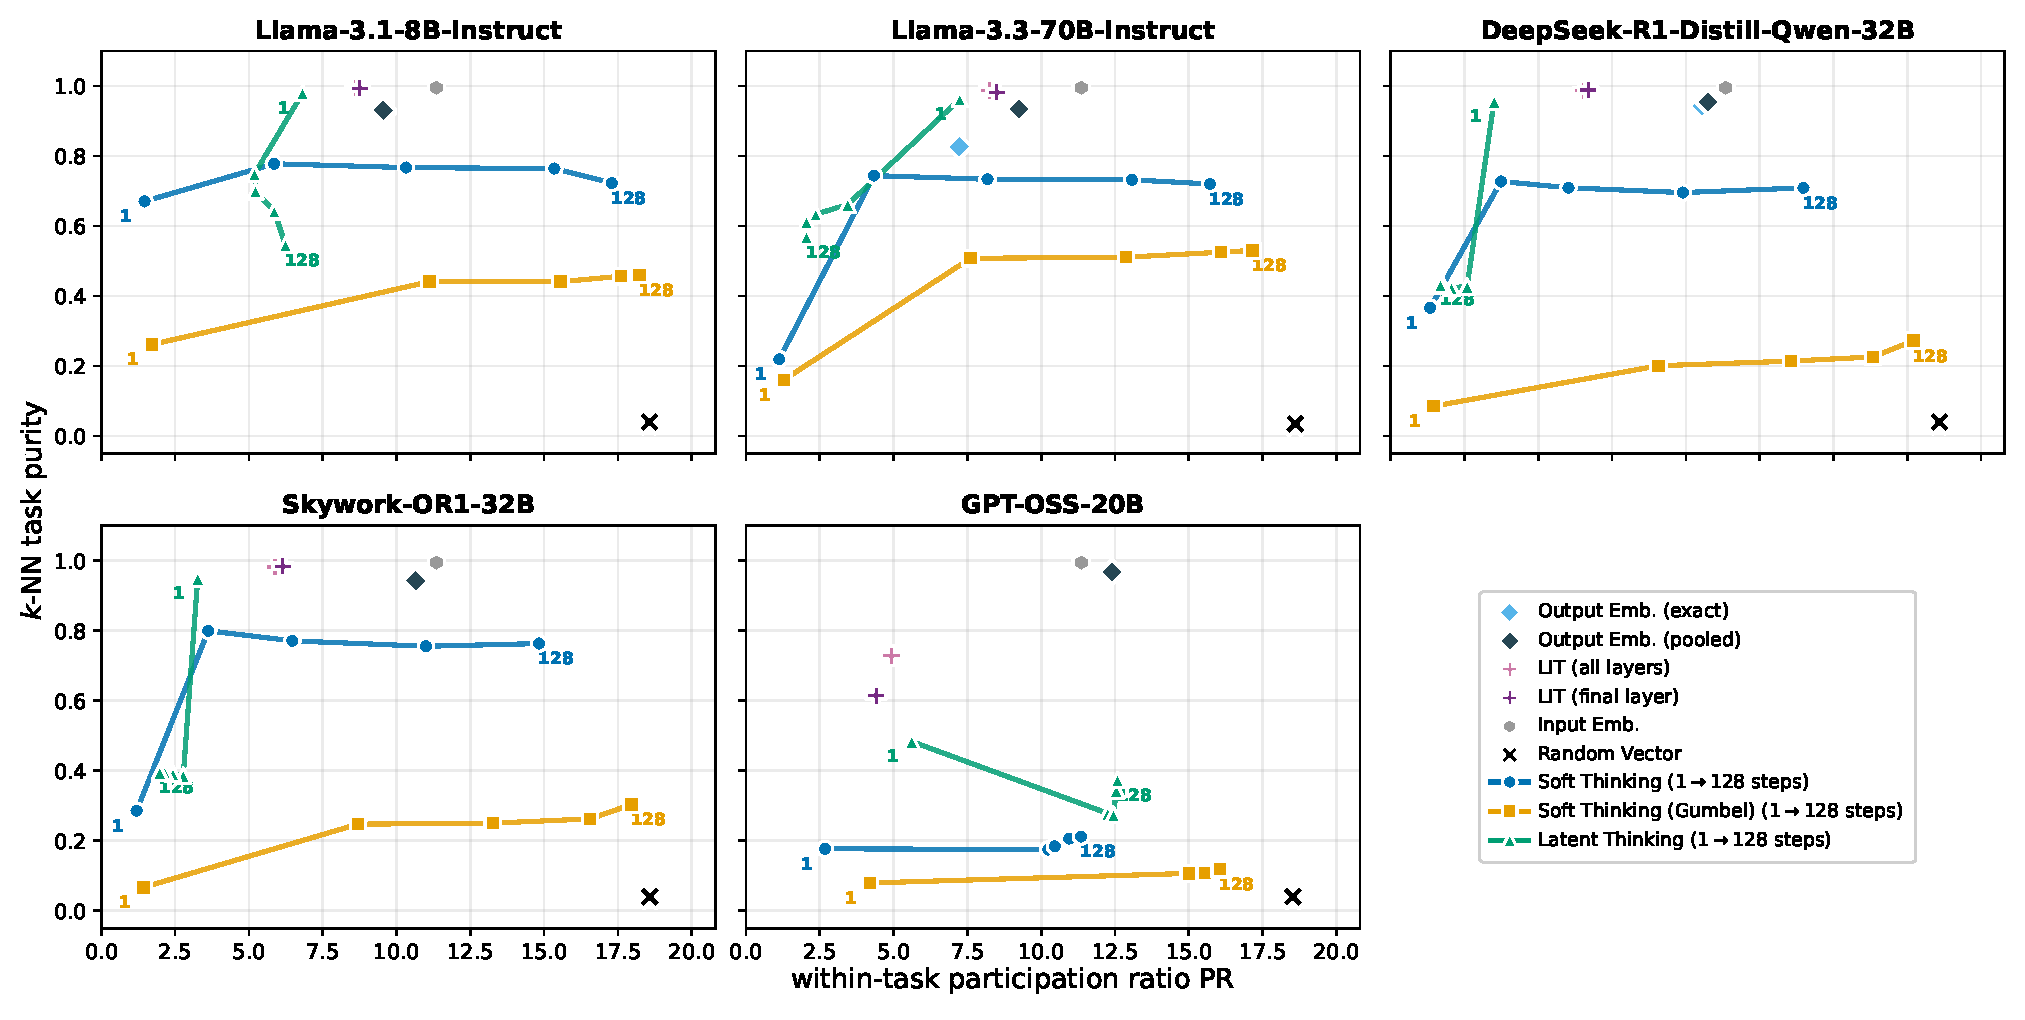
\includegraphics[width=0.98\linewidth]{figures/pdf/geom_summary_multi.pdf}
  \caption{Each candidate placed on the $(\mathrm{PR}, k\text{-NN purity})$ plane, one panel per LLM. Solid lines trace thinking-family trajectories as the step count grows from $1$ to $128$. Candidates further to the upper right are preferable: higher $\mathrm{PR}$ indicates a within-task subspace spread across more directions, and higher $k$-NN purity indicates that nearest neighbours are drawn from the same task.}
  \label{fig:geom-summary}
\end{figure}
